% title: response.tex
% description: Response to eLife Reviewers
% author: twab

% USAGE: 
% to compile this document:
%    R  >>> knitr::knit("response.Rnw")
%    sh >>> pdflatex response.tex


%% R --------------------------------------------------------------------------



%% latex document setup -------------------------------------------------------

\documentclass[11pt]{elife}\usepackage[]{graphicx}\usepackage[]{color}
% maxwidth is the original width if it is less than linewidth
% otherwise use linewidth (to make sure the graphics do not exceed the margin)
\makeatletter
\def\maxwidth{ %
  \ifdim\Gin@nat@width>\linewidth
    \linewidth
  \else
    \Gin@nat@width
  \fi
}
\makeatother

\definecolor{fgcolor}{rgb}{0.345, 0.345, 0.345}
\newcommand{\hlnum}[1]{\textcolor[rgb]{0.686,0.059,0.569}{#1}}%
\newcommand{\hlstr}[1]{\textcolor[rgb]{0.192,0.494,0.8}{#1}}%
\newcommand{\hlcom}[1]{\textcolor[rgb]{0.678,0.584,0.686}{\textit{#1}}}%
\newcommand{\hlopt}[1]{\textcolor[rgb]{0,0,0}{#1}}%
\newcommand{\hlstd}[1]{\textcolor[rgb]{0.345,0.345,0.345}{#1}}%
\newcommand{\hlkwa}[1]{\textcolor[rgb]{0.161,0.373,0.58}{\textbf{#1}}}%
\newcommand{\hlkwb}[1]{\textcolor[rgb]{0.69,0.353,0.396}{#1}}%
\newcommand{\hlkwc}[1]{\textcolor[rgb]{0.333,0.667,0.333}{#1}}%
\newcommand{\hlkwd}[1]{\textcolor[rgb]{0.737,0.353,0.396}{\textbf{#1}}}%
\let\hlipl\hlkwb

\usepackage{framed}
\makeatletter
\newenvironment{kframe}{%
 \def\at@end@of@kframe{}%
 \ifinner\ifhmode%
  \def\at@end@of@kframe{\end{minipage}}%
  \begin{minipage}{\columnwidth}%
 \fi\fi%
 \def\FrameCommand##1{\hskip\@totalleftmargin \hskip-\fboxsep
 \colorbox{shadecolor}{##1}\hskip-\fboxsep
     % There is no \\@totalrightmargin, so:
     \hskip-\linewidth \hskip-\@totalleftmargin \hskip\columnwidth}%
 \MakeFramed {\advance\hsize-\width
   \@totalleftmargin\z@ \linewidth\hsize
   \@setminipage}}%
 {\par\unskip\endMakeFramed%
 \at@end@of@kframe}
\makeatother

\definecolor{shadecolor}{rgb}{.97, .97, .97}
\definecolor{messagecolor}{rgb}{0, 0, 0}
\definecolor{warningcolor}{rgb}{1, 0, 1}
\definecolor{errorcolor}{rgb}{1, 0, 0}
\newenvironment{knitrout}{}{} % an empty environment to be redefined in TeX

\usepackage{alltt}
\usepackage{amsmath}
\usepackage{amssymb}
\usepackage{amsthm}
\usepackage{ragged2e}
\usepackage{caption}
\usepackage{fancyhdr}
\usepackage{graphicx}
\usepackage{titlesec}
\usepackage{blkarray}
\usepackage{csquotes}

\graphicspath{ {./figs/} }


\title{Supplementary Methods\\
\small{Genetic Disruption of WASHC4 Drives Endo-lysosomal Dysfunction and \\
Cognitive-Movement Impairments in Mice and Humans}}

\author[1\authfn{0}]{Jamie Courtland}
\author[1\authfn{0}]{Tyler W. A. Bradshaw}
\author[2]{Greg Waitt}
\author[2,3]{Erik J. Soderblom}
\author[2]{Tricia Ho}
\author[4]{Anna Rajab}
\author[5]{Ricardo Vancini}
\author[2\authfn{1}]{Il Hwan Kim}
\author[6]{Ting Huang}
\author[6]{Olga Vitek}
\author[3]{Scott H. Soderling}

\affil[1]{Department of Neurobiology, Duke University School of Medicine, 
Durham, NC 27710, USA}
\affil[2]{Proteomics and Metabolomics Shared Resource, 
Duke University School of Medicine, Durham, NC 27710, USA}
\affil[3]{Department of Cell Biology, Duke University School of Medicine, 
Durham, NC 27710, USA}
\affil[4]{Burjeel Hospital, VPS Healthcare, Muscat, Oman}
\affil[5]{Department of Pathology, Duke University School of Medicine, 
Durham, NC 27710, USA}
\affil[6]{Khoury College of Computer Sciences, Northeaster University,
Boston, MA 02115, USA}

\contrib[\authfn{0}]{These authors contributed equally to this work.}
\presentadd[\authfn{1}]{Department of Anatomy and Neurobiology, 
University of Tennessee Health Science Center, Memphis, TN 38163, USA}

\corr{jlc123@duke.edu}{JC}
\corr{tyler.w.bradshaw@duke.edu}{TWAB}
\corr{greg.waitt@duke.edu}{GW}
\corr{erik.soderblom@duke.edu}{EJB}
\corr{tricia.ho@duke.edu}{TH}
\corr{drannarajab@gmail.com}{DR}
\corr{ricardo.vancini@duke.edu}{RV}
\corr{ikim9@uthsc.edu}{IK}
\corr{huang.tin@northeastern.edu}{TH}
\corr{o.vitek@northeastern.edu}{OV}
\corr{scott.soderling@duke.edu}{SHS}


\setlength{\abovedisplayskip}{3pt}
\setlength{\belowdisplayskip}{3pt}


%% main -----------------------------------------------------------------------
\IfFileExists{upquote.sty}{\usepackage{upquote}}{}
\begin{document}

\maketitle

\renewcommand{\abstractname}{Summary}
\begin{abstract}

Here we address concerns about the statistical validity of our previous approach
to assess differential protein abundance in the \textbf{WASH-iBioID} and
\textbf{SWIP-TMT} proteomics datasets. Our previous approach depended
upon the R package \texttt{edgeR}. We used \texttt{edgeR} to perform
both protein- and module-level inference---assessing differential
abundance of individual proteins as well as protein groups in
SWIP\textsuperscript{P1019R} mouse brain. \texttt{edgeR} utilizes a
negative binomial (NB) generalized linear model (GLM) framework
originally developed for analysis of RNA-Seq data.  Previously, we
failed to fully consider the validity of \texttt{edgeR's} NB assumption
for proteomics data. We evaluate the goodness-of-fit of the NB GLM for
our TMT dataset and find evidence of a lack-of-fit.  Thus, we revise our
statistical approach and reanalyze our data, making use of Huang
\textit{et al.}'s recently published R package \texttt{MSstatsTMT}.
\texttt{MSstatsTMT} utilizes linear-mixed models to capture the complex
sources of variation in TMT proteomics experiments and evaluate
protein-level differential abundance.  We extend the flexible
linear-mixed model (LMM) framework used by \texttt{MSstatsTMT} to
re-evaluate both protein- and module-level statistical comparisions in
our SWIP-TMT spatial proteomics dataset.\\

\end{abstract}

\newpage


\section{Lack-of-fit of the NB model}

Our previous approach can be summarized as the \textit{Sum + IRS} method \citep{Huang2020}.
Following protein summarization (by summing its features) and internal
reference scaling (IRS) normalization \citep{Plubell2017},  we applied
\texttt{edgeR} \citep{McCarthy2012} to assess differential abundance of individual proteins and
protein-groups.  The use of \texttt{edgeR} for protein-level comparisons was
based on work by Plubell \textit{et al.} who describe IRS normalization and the
use of \texttt{edgeR} for statistical testing in TMT MS experiments
(Plubell2017).  We failed however, to consider the overall adequacy of the NB
GLM model for our TMT proteomics data.

Statisitical inference in \texttt{edgeR} is performed for each gene or protein 
using a negative binomial framework. The data are assumed to 
be adequately described by a NB distribution parameterized by a dispersion 
parameter, $\phi$. Practically, the dispersion parameter accounts for the
observed mean-variance relationship in proteomics and transcriptomics data.

As signal intensity in protein MS is fundamentally related to the number of ions generated from
an ionized, fragmented protein, we incorrectly inferred that TMT
mass spectrometry data can be modeled as negative binomial count data. Based on
this assumption, we justified the use of \texttt{edgeR}.  Here, we reconsider
the overall adequacy of the \texttt{edgeR} NB GLM model for TMT MS data.

To evaluate the overall adequacy of the \texttt{edgeR} model, we plot the
residual protein deviance statistics of all proteins against their theoretical
normal quantiles in a quantile-quantile (QQ) plot (FIG:gof).  The QQ plot
addresses the question of how similar the observed data are to the theoretical
distribution.  A linear relationship between the observed and theoretical
values is an indicator of goodness-of-fit.  Deviation from this linear trend is
evidence of a lack-of-fit.

Following protein summarization and normalization with \texttt{MSstatsTMT}, the
SWIP-TMT data were fit with a NB GLM using \texttt{edgeR::glmFit}. FIG:gof
illustrates the divergence of the observed and theoretical quantiles for our
SWIP-TMT dataset fit with \texttt{edgeR's} NB GLM. Given our experimental
design, \texttt{MSstatsTMT} fits an appropriate linear-mixed model expressing
the major sources of variation in our experiment.  The quantile-quantile plot in
FIG:gof indicates that the data are well described by \texttt{MSstatsTMT's} LMM,
which does not depend upon the negative binomial assumption.

% NOTE: we also assess the gof of the Khan TMT dataset using the IRS method and
% observe a similar lack of fit for the NB GLM.
%These plots emphasize the overall lack-of-fit for proteomics data fit with the \texttt{edgeR} model.\\ 

\section{Protein-wise LMMs for MSstatsTMT}

The strength of linear mixed-models lies in their flexibility. In LMMs 
the response variable is taken to be a function of both fixed- and random-effects. 
If the set of possible levels of a covariate is fixed and reproducible, then the
factor is modeled as a fixed-effect parameter.  In contrast, if the levels of an
observation reflect a sampling of the set of all possible levels, then the
covariate is modeled as a random-effect.  Random or mixed-effects represent
categorical variables that reflect experimental or observational units within
the dataset (Bates2015).  As such, mixed-effect parameters account for the
variation occurring among the lower levels of an upper level unit in the data
(Bates2015).  Using LMMs we can untangle the variance attributable to the
biological effect we are interested in from the experimental and biological
covariates which mask this response.

Huang \textit{et al.} created \texttt{MSstatsTMT}, an R package for data
normalization and hypothesis testing in multiplex TMT proteomics experiments. 
They outline a common vocabulary for describing the experimental design of 
a general TMT mass spectrometry experiment. An experiment consists of 
\texttt{m = 1} ... \texttt{M}\ concatenations of isobarically labeled samples or
\texttt{Mixtures}.  This mixture is then analyzed by the mass spectrometer in a
mass spectrometry \texttt{Run}.  This mixture is often fractionated into
multiple liquid chromotography \texttt{Fractions} to decrease sample complexity,
and thereby increase the depth of proteome coverage.  Within a mixture, each of
the unique TMT channels is dedicated to the analysis of \texttt{c = 1} ...
\texttt{C}\ individual biological or treatment \texttt{Conditions}.  There may
then be \texttt{b = 1} ... \texttt{B}\ biological replicates or
\texttt{Subjects}. Finally, a single TMT mixture may be repeatedly analyzed in
\texttt{t = 1} ... \texttt{T}\ technical replicate mass spectrometry runs.

Equation \ref{eq:full} is a LMM describing protein abundance as a function of
the major sources of variation  in a general TMT experiment composed of
\texttt{M} mixtures, \texttt{T} technical replicates of mixture, \texttt{C}
conditions, and \texttt{B} biological subjects.
\begin{equation} % eq:full
  \label{eq:full} 
	Y_{mcbt} = \mu + Mixture_m + TechRep(Mixture)_{m(t)} + Condition_c + 
	Subject_b + \epsilon_{mcbt}\\
\end{equation}

\begin{equation}
  \begin{gathered}
    \label{eq:constraints}
	\sum_{c=1}^{C} Condition_c = 0 \\
	Subject_{mcb} \stackrel{iid}{\sim} N(0,\sigma^2_S) \\
	Mixture_m \stackrel{iid}{\sim} N(0,\sigma^2_M) \\
	TechRep(Mixture)_{t(m)} \stackrel{iid}{\sim} N(0,\sigma^2_T) \\
	\epsilon{mtcb} \stackrel{iid}{\sim} N(0,\sigma^2) \\
  \end{gathered}
\end{equation}

The model's constraints \ref{eq:constraints} distinguish fixed- and mixed-effect
components of variation in the response, $Y_{mcbt}$. \texttt{Mixture} is a
mixed-effect and represents variation between different TMT mixtures. By definition
mixed-effects are assumed to be normally and independently distributed (\texttt{iid}). 
The term \texttt{TechRep(Mixture)} represents random variation between
replicates of a single MS \texttt{Run}. \texttt{Subject} cooresponds
to each unique biological replicate and represents biological variation among
the levels of the fixed-effect \texttt{Condition}. The term
$\epsilon_{mtcb}$, is a mixed-effect representing both biological and technical
variation, quantifying any remaining error. If a component of the model is not
estimable, then it is removed.  For example, if there is no technical
replication of mixture \texttt{(T=0)}, 
then the model is reduced to equation \ref{eq:reduced}.
\begin{equation} % NOTE: dont put blank lines above equations!
	\label{eq:reduced} % equation -- reduced
	Y_{mcbt} = \mu + Mixture_m + Condition_c + Subject_b + \epsilon_{mcb}
\end{equation}


\section{SWIP-TMT Experimental Design}

Each 16-plex TMT mixture contains seven repeated measurements made from each
biological subject (FIG:design).  To account for this repeated measures
design, we should include the random-effect term \texttt{Subject}.
In our experiment however, \texttt{Mixture} is confounded with \texttt{Subject}.
In each \texttt{Mixture} we analyzed all seven \texttt{BioFractions} from a
single Control and Mutant mouse. Thus we can choose to
account for the effect of \texttt{Mixture} or \texttt{Subject}, but not both. We
choose to account for variability of \texttt{Mixture} based on the assumption
that the variance associated with this experimental batch effect is greater than
the intra-Subject error inherent in the repeated measures of each subject.
In our experiment, the fixed-effect term \texttt{Condition} in equation
\ref{eq:reduced} represents the fourteen combinations of \texttt{Genotype} and
\texttt{BioFraction} obtained from subcellular fractionation of Control and
SWIP\textsuperscript{P1019R} Mutant mouse brains. We refer to these as a
\texttt{BioFraction} to distinguish them from an MS \texttt{Fraction}. 
We omit the un-estimable terms \texttt{TechRep(Mixture)} and \texttt{Subject}
from equation (\ref{eq:full}). The reduced model is equation \ref{eq:fx0}.
\begin{equation}
	\label{eq:fx0}
	Y_{mcbt} = \mu + Mixture_m + Condition_c + \epsilon_{mcb}
\end{equation}


\section{Statistical inference with SstatsTMT}

\texttt{MSstatsTMT} performs protein-wise comparisons between pairs of 
\texttt{Conditions} by comparing the estimates obtained from the fit LMM. 
We are interested in testing the hypothesis:
\begin{equation}
	\label{eq:null} % equation -- null
	H0 : l^T * \beta = 0. 
\end{equation}

Where $l^T$ is a vector of $\sum=1$ specifying the positive and negative
coefficients of a contrast. $\beta$ is the model-based estimates of
\texttt{Condition}.  The null hypothesis (\ref{eq:null}) is that the fold
change, $\l^T * \beta$, is 0.  A test statistic for such a two-way contrasts is
given by Kutzenova \textit{et al.,} (Kutzenova2017):
\begin{equation} 
	\label{eq:tstatistic} % equation -- tstatistic
	t = \frac{l^T \hat{\beta}}{\sqrt{l \sigma^2 \hat{V} l^T}}
\end{equation}

We obtain the models estimates $\hat{\beta}$, error $\sigma^2$, and
variance-covariance matrix $\hat{V}$ from the model fitted by restricted maximum
likelihood (Bates2015). Given a contrast, $l^T$, the numerator of equation
(\ref{eq:tstatistic}) is the fold change of a comparison.  The product of
$\sigma^2$ and $\hat{V}$ is the scaled variance-covariance matrix describing
error estimates of the model's fixed- and mixed-effect parameters.  Together the
denominator represents the standard error of the comparison. The degrees of
freedom for the contrast are derived using the Satterthwaite moment of
approximation method (Satterthwaite1946, Kutzenova2017).  Finally, a p-value is
calculated given the t-statistic and degrees of freedom.  P-values for the
protein-wise tests are adjusted using the Benjamini-Hochberg FDR method
(Benjamini1995,Huang2020).\\


\section{Protein-level comparisons}

Following data preprocessing, summarization, and normalization, statistical
inference by \texttt{MSstatsTMT} is performed by (1) fitting each protein in the
dataset with an appropriate LMM and then (2) given the fitted model, assessing a
contrast of interest. Using \texttt{MSstatsTMT} we assesssed two types of
protein comparisons:
\begin{itemize}
	\item \texttt{intra-BioFraction} comparisons
	\item \texttt{Mutant-Control} contrast
\end{itemize}

\texttt{Intra-BioFraction} comparisons are the seven pairwise comparisons of 
Control and Mutant protein abundance for each subcellular
\texttt{BioFraction}. We also assessed differential abundance for the 
overall \texttt{Mutant-Control} comparison. Each of these contrasts is 
represented by a vector, $l^T$, which specifies a comparison between 
coefficients of \texttt{Condition} in the LMM (\ref{eq:fx0}).
FIG:contrasts illustrates a matrix defining all eight unique comparisons.

\texttt{MSstatsTMT} attempts to automatically parse the experimental design and
fit the appropriate LMM to each protein in the dataset. In order to understand 
and extend the function of \texttt{MSstatsTMT}, 
we extracted \texttt{MSstatsTMT's} core model-fitting and statistical 
testing steps and illustrate them here.

At the core of the model fitting-step is the R package \texttt{lme4} which
implements mixed-effects models with its function \texttt{lme4::lmer}(Bates2015). The
package \texttt{lmerTest} extends \texttt{lme4's} functionality and enables the
computation of Sattertwaite degrees of freedom (Kutzenova2017). As an example,
we illustrate the analysis of WASHC4. First, we fit the model (\ref{eq:fx0}) to
a subset of the data, the data for WASHC4.\\




%% latex -----------------------------------------------------------------------

The model's estimates ($\beta$) represent our best estimate of the mean protein
abundance in the fourteen conditions of \texttt{Genotype:BioFraction}. 
To illustrate an \texttt{intra-BioFraction} comparison, we 
define a contrast comparing the \texttt{Mutant:F7} and \texttt{Control:F7}
conditions. The function \texttt{lmerTestContrast} performs the statstical comparison given
a fitted model and a contrast vector defining a comparison between the models
coefficients. While the work done by this function 
is the same as the work done internally by \texttt{MSstatsTMT's}
\texttt{groupComparisonsTMT} function, \texttt{lmerTestContrast} is more
flexible. Provided the correct contrast, we also easily assess the overall
\texttt{Mutant-Control} comparison.\\


\section{Module-level comparisons}

We wish to extend the LMM framework developed by \texttt{MSstatsTMT} to perform 
inference at the level of protein groups or modules.
That is, for module-level comparisons, we are interested in the overall effect 
of Genotype on a group of proteins. Where modules are groups of covarying 
proteins which represent biological niches defined by proteins that 
localized together in subcellular space.\\

Here we hypothesize that the proteins within a module, which are a subset of the
overall proteome,  are a part of a common group, a module, with a common mean
effect. Proteins within a module are correlated observations which we model as a
mixed-effect as we are primarily interested in making inference about the
overall distribution of the responses for a module rather than among its
sublevels. The following LMM includes the additional mixed effect term
\texttt{Protein}, capturing variance among a module's constintuent proteins.
\begin{equation} 
  \begin{gathered}\label{eq:fx1} % equation -- fx1
	Y_{mcbt} = \mu + Mixture_m + Condition_c + Protein_p + \epsilon_{mcb}\\
	Protein_p \stackrel{iid}{\sim} N(0,\sigma^2_P) \\
  \end{gathered}
\end{equation}

The term \texttt{Protein} in equation \ref{eq:fx1} quantifies the variance
$\sigma_P$ attributable to all proteins in a module.  As a means of example, we
demonstrate an ideal module, by fitting LMM (\ref{eq:fx1}) to the five WASH
complex proteins.  As before, we calculate the coefficient of determination for
LMM's with the \texttt{r.squaredGLMM} function (WangMerkel2018).\\


\section{LMM Goodness-of-fit}

Again, we consider the total variance explained as a measure of the model's
overall quality. Our model explains 89.2\% of the total variance among these
five proteins. The fixed-effect term \texttt{Genotype:BioFraction} explains the
majority of variance ($R^2_m=0.762$). The remaining 13.0\% variance is
attributable to a combination of mixed-effects \texttt{Mixture} and
\texttt{Protein} as well as the residual variance. We assess the overall
\texttt{Mutant-Control} difference between responses of of 'Mutant' and Control
groups as before. The R package \texttt{variancePartition} enables us to
calculate the percent variance explained by a LMM's parameters. To do so, it
expects all terms to be mixed-effects. FIG:variance.

It is useful to consider the goodness-of-fit of our LMM. A straight forward
measure of a LMM's quality is the Nakagawa coefficient of 
determination (Nakagawa2013,Nakagawa2017). Nakagawa's conditional $R^2$ is 
interpreted as the total variance explained by a LMM ($R^2_{total}$).
The marginal $R^2$ is interpreted as the variance explained by the LMM's 
fixed-effects ($R^2_{fixed}$). We implment Nakagawa's coeffficient of 
determination using the \texttt{r.squaredGLMM} function taken from the 
\texttt{MuMin} package (WangMerkel2018).
The total variation explained, $R^2_{c}$, for the LMM fit to WASHC4 is 
\texttt{0.949}. The variance explained by fixed-effects, represents a large
fraction of this total ($R^2{m}$=0.935). It follows that 1.5\% of the remaing
variance is attributable to residuals and the mixed-effect \texttt{Mixture}.\\

We can see that the majority of the variance explained by the LMM fit to the
WASH complex is attributable to \texttt{Genotype}. The mixed-effect terms
\texttt{Protein} and \texttt{Mixture} account for a small fraction of the 
overall variance explained by the model.

As our overall goal is to identify groups or modules of proteins that strongly
covary together, our clustering approach should maximize the variance explained
by a module's fixed-effect parameters (Genotype + BioFraction) while minimizing 
the variance among its individual proteins. 
An ideal module is a perfect summary of its protein constituents, 
$PVE_{Protein}=0$. We use this idea of a module's quality to supervise our 
clustering approach.
\begin{equation}
	Q_{M}=\frac{PVE_{Genotype} + PVE_{BioFraction}}{PVE_{Protein}}
\end{equation}


\section{Network Construction}

Using our SWIP-TMT dataset, we aim to identify modules or groups of
proteins that covary together across subcellular space. Prior to building the
co-variation network, other sources of variation should be removed. Although
\texttt{MSstatsTMT} handles the batch effect inherent in experiments with
multiple TMT mixtures, it is necessary to remove this effect prior to building
the network. We removed the effect of \texttt{Mixture} using
\texttt{limma::RemoveBatchEffect}. These adjusted data are used for network
construction and plotting but not statistical modeling.

Prior to network construction, we removed protein models with poor fit 
($R^2_{total}<0.7$; n=791 proteins). Removing this noisey proteins facilitation
module identification and improves overall module quality.

The final network was constructed using data from both Control and Mutant 
samples after adjusting for batch (Mixture). The final dataset included 
42 samples and 6,119 proteins. The protein covariation network was build by
calculating the Pearson correlation for all pairwise comparisons of proteins.

We performed network enhancement to remove biological noise from the network
prior to clustering. This step is essential in large, and dense networks for
module detection. Network enhancement reweights the
network's edges and has the overall effect of making the network sparse.
Conceptually this step is related to the soft-thresholding approach taken by
WGCNA or WPCNA analysis workflows (REFS), but has the benefit of not assuming
that the network has an overall scale free topology.  Without reweighting or
enhancing the network, most extant clustering algorithms fail to detect
communities in the dataset.  Network enhancment has the effect of making the
network sparse and facilitates the identification of network structure.\\

\section{Code}

% R code to do something else

\begin{knitrout}
\definecolor{shadecolor}{rgb}{0.969, 0.969, 0.969}\color{fgcolor}\begin{kframe}
\begin{alltt}
\hlcom{# load dependencies}
\hlkwd{library}\hlstd{(dplyr)}
\hlkwd{library}\hlstd{(lmerTest)}

\hlcom{# load SwipProteomics}
\hlkwd{data}\hlstd{(swip)}
\hlkwd{data}\hlstd{(msstats_prot)}

\hlcom{# formula to be fit to WASHC4, aka SWIP:}
\hlstd{fx0} \hlkwb{<-} \hlstr{'Abundance ~ 0 + Genotype:BioFraction + (1|Mixture)'}

\hlcom{# fit the LMM}
\hlstd{fm0} \hlkwb{<-} \hlkwd{lmer}\hlstd{(fx0, msstats_prot} \hlopt \hlkwd{subset}\hlstd{(Protein} \hlopt{==} \hlstd{swip))}

\hlcom{# examine the model's summary}
\hlkwd{summary}\hlstd{(fm0,} \hlkwc{ddf} \hlstd{=} \hlstr{"Satterthwaite"}\hlstd{)}
\end{alltt}
\begin{verbatim}
## Linear mixed model fit by REML. t-tests use Satterthwaite's method [
## lmerModLmerTest]
## Formula: fx0
##    Data: msstats_prot %>% subset(Protein == swip)
## 
## REML criterion at convergence: 3.7
## 
## Scaled residuals: 
##     Min      1Q  Median      3Q     Max 
## -1.5030 -0.6089 -0.1463  0.7474  1.4302 
## 
## Random effects:
##  Groups   Name        Variance Std.Dev.
##  Mixture  (Intercept) 0.009596 0.09796 
##  Residual             0.034418 0.18552 
## Number of obs: 42, groups:  Mixture, 3
## 
## Fixed effects:
##                                Estimate Std. Error      df t value Pr(>|t|)    
## GenotypeMutant:BioFractionF4     5.4043     0.1211 17.3059   44.62   <2e-16 ***
## GenotypeControl:BioFractionF4    6.7110     0.1211 17.3059   55.41   <2e-16 ***
## GenotypeMutant:BioFractionF5     5.5674     0.1211 17.3059   45.96   <2e-16 ***
## GenotypeControl:BioFractionF5    6.9456     0.1211 17.3059   57.34   <2e-16 ***
## GenotypeMutant:BioFractionF6     5.6402     0.1211 17.3059   46.56   <2e-16 ***
## GenotypeControl:BioFractionF6    7.2401     0.1211 17.3059   59.77   <2e-16 ***
## GenotypeMutant:BioFractionF7     5.6317     0.1211 17.3059   46.49   <2e-16 ***
## GenotypeControl:BioFractionF7    7.3211     0.1211 17.3059   60.44   <2e-16 ***
## GenotypeMutant:BioFractionF8     5.4928     0.1211 17.3059   45.35   <2e-16 ***
## GenotypeControl:BioFractionF8    7.1296     0.1211 17.3059   58.86   <2e-16 ***
## GenotypeMutant:BioFractionF9     5.7810     0.1211 17.3059   47.73   <2e-16 ***
## GenotypeControl:BioFractionF9    6.9545     0.1211 17.3059   57.41   <2e-16 ***
## GenotypeMutant:BioFractionF10    5.7844     0.1211 17.3059   47.76   <2e-16 ***
## GenotypeControl:BioFractionF10   7.6187     0.1211 17.3059   62.90   <2e-16 ***
## ---
## Signif. codes:  0 '***' 0.001 '**' 0.01 '*' 0.05 '.' 0.1 ' ' 1
\end{verbatim}
\end{kframe}
\end{knitrout}


\section{References}

\bibliography{bibliography}


\section{Figures}

% title: figures.tex
% description: supplemental latex figures
% author: twab


\begin{figure}[h] % figure -- gof
	\begin{fullwidth}
		\begin{center}
		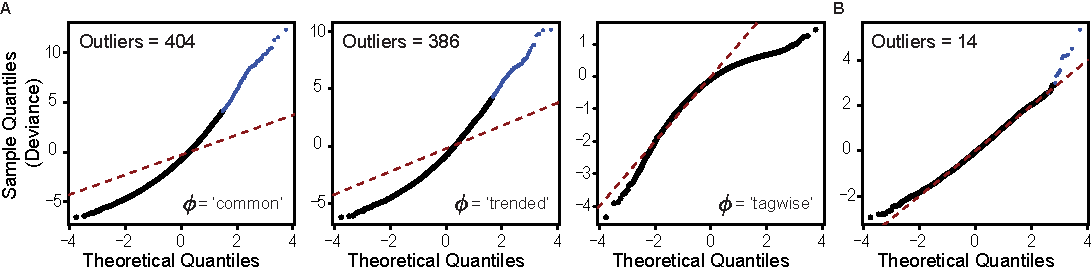
\includegraphics[width=0.9\paperwidth,keepaspectratio]{gof}
		\caption{\textbf{Goodness-of-fit of the \texttt{edgeR} model for
		TMT proteomics data.} The overall
		adequacy of the NB GLM fit to the data were assessed 
		by plotting the residual deviance for all proteins as a 
		quantile-quantile plot (McCarthy \textit{et al.}, (2012)). 
		\textbf{(A)} The normalized protein data were fit with a 
		binomal generalized linear model of the form: 
		\texttt{log2(Intensity)} $\sim$ \texttt{Mixture + Condition}.
		Where \texttt{Mixure} is an additive blocking factor that 
		accounts for variablity between experiments.  The NB framework
		used by \texttt{edgeR} utilizes a dispersion parameter,
		$\psi$, to model mean-variance relationships in the data
		in three different ways.
		The dispersion parameter can take the form of: 'common', 'trended', and 'tagwise'. 
		We plot the deviance
		statistics for the data fit with each of
		the three disperions parameters against their 
		theoretical normal quantiles using the \texttt{edgeR::gof}
		function. \textbf{(B)} For analysis with \texttt{MSstatsTMT},
		the normalized protein data were fit with a linear mixed-effects 
		model (LMM) of the form: 
		\texttt{Abundance} $\sim$ \texttt{0 + Condition + (1|Mixture)}. 
		Where \texttt{Mixture} represents the mixed-effect
		of \texttt{Mixture}. The residual deviance and degrees of 
		freedom were extracted from the fitted models, z-score
		normalized, and plotted as in (A). Proteins with a significantly 
		poor fit are indicated as outliers in blue 
		(Holm-adjusted P-value $<$ 0.05).}
		\label{fig:gof}
	\end{center}
	\end{fullwidth}
\end{figure}

\newpage

\begin{figure}[h] %% ./figs/khan.pdf
  \begin{fullwidth}
  \begin{center}
	  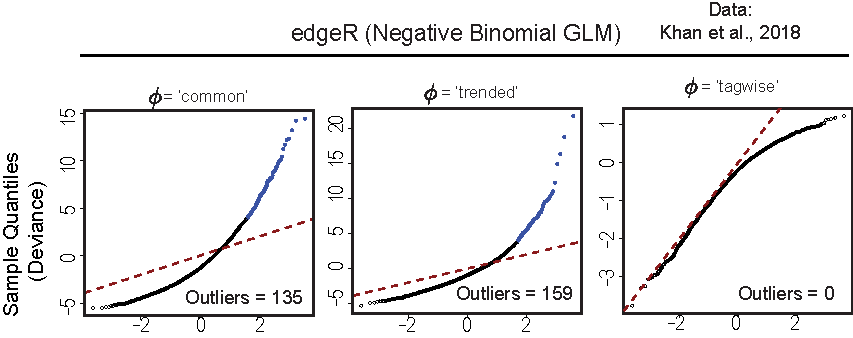
\includegraphics[width=0.9\paperwidth,keepaspectratio]{khan}
	  \caption{\textbf{Goodness-of-fit for the edgeR NB GLM for the Khan
	  \textit{et al}, (2018) dataset.} } % EOC
	  \label{fig:khan}
  \end{center}
  \end{fullwidth}
\end{figure}

\newpage


\begin{figure}[h] %% figure -- ./figs/impute.pdf
  \begin{fullwidth}
  \begin{center}
	  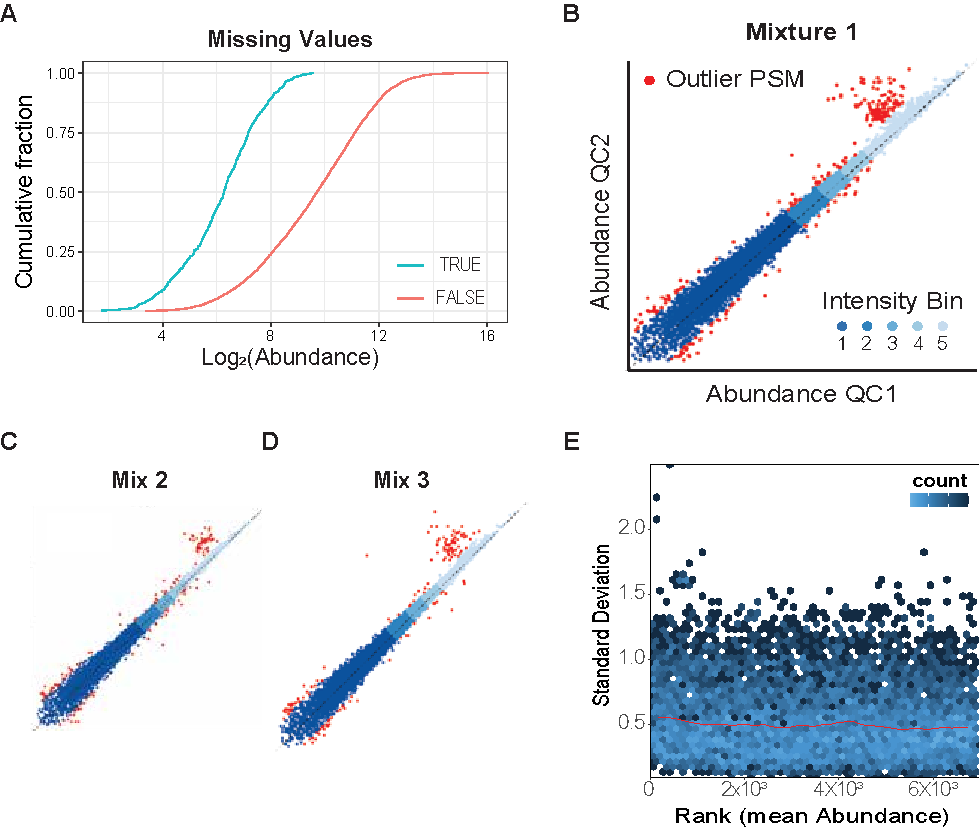
\includegraphics[width=0.9\paperwidth,keepaspectratio]{impute}
	  \caption{\textbf{Missing value imputation and PSM outlier removal.}
	  \textbf{A} \textbf{B} \textbf{C} \textbf{D} }
	  \label{fig:impute}
  \end{center}
  \end{fullwidth}
\end{figure}

\newpage


\begin{figure}[h] %% figure -- normalization.pdf
  \begin{fullwidth}
  \begin{center}
	  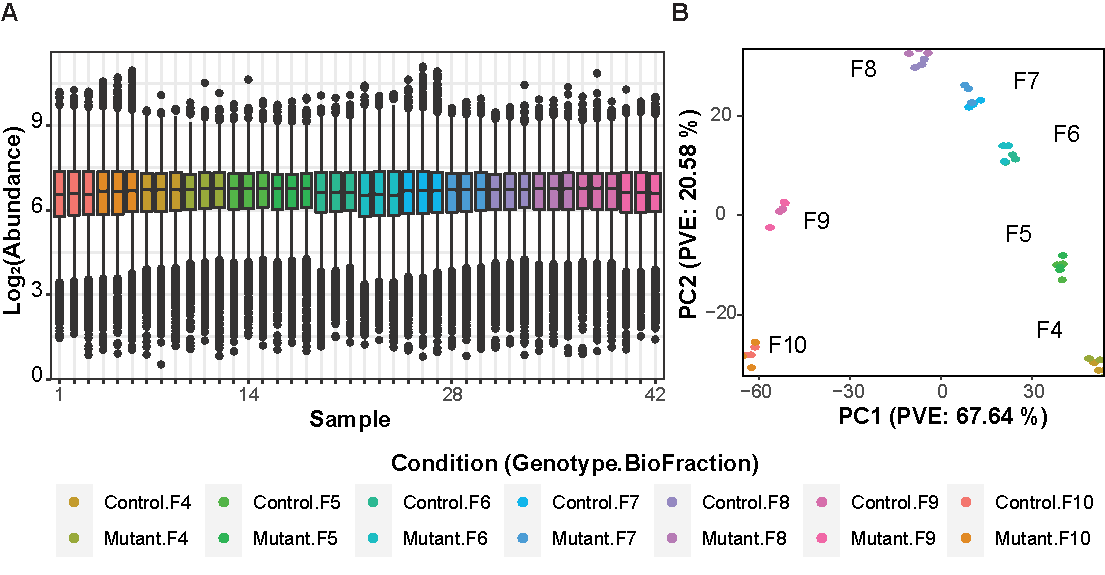
\includegraphics[width=0.9\paperwidth,keepaspectratio]{normalization}
	  \caption{\textbf{Data Normalization and PCA.} \textbf{A} \textbf{B} }
	  \label{fig:normalization}
  \end{center}
  \end{fullwidth}
\end{figure}

\newpage


\begin{figure}[h] %% figure [x] -- washc4.pdf
  \begin{fullwidth}
  \begin{center}
	  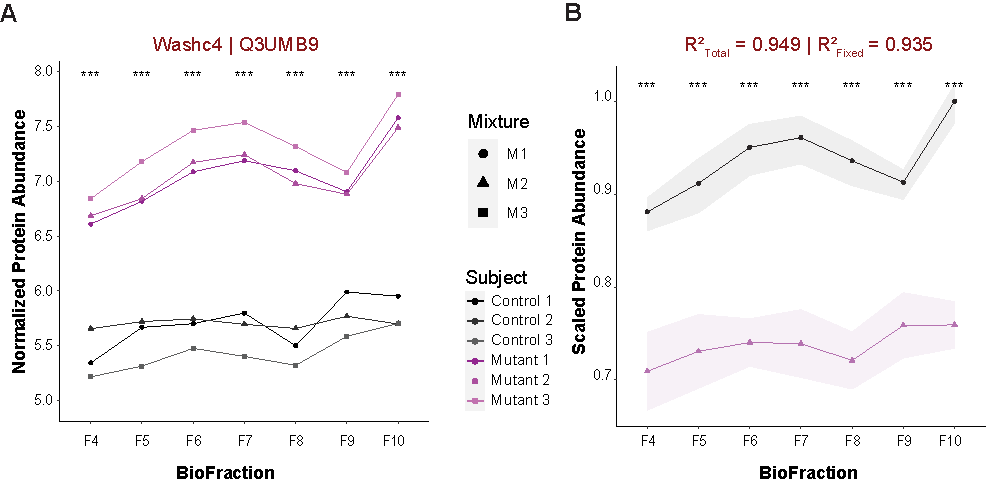
\includegraphics[width=0.9\paperwidth,keepaspectratio]{washc4}
	  \caption{\textbf{Data Normalization and PCA.} \textbf{A} \textbf{B} }
	  \label{fig:washc4}
  \end{center}
  \end{fullwidth}
\end{figure}

\newpage




\begin{figure}[h] %% figure x -- design 
  \begin{fullwidth}
  \begin{center}
	  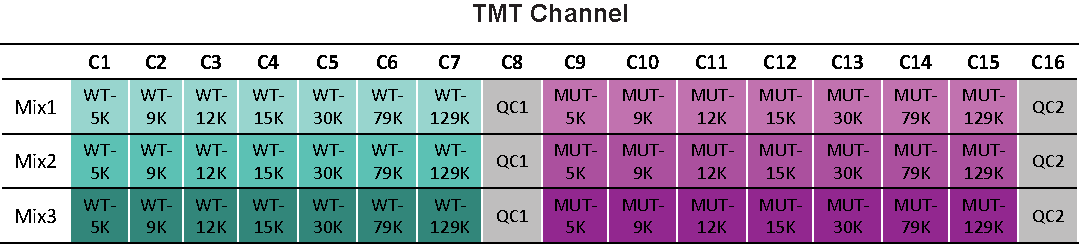
\includegraphics[width=0.9\paperwidth,keepaspectratio]{design}
	  \caption{\textbf{Experimental Design.} We performed three 16-plex TMT
	  experiments. Each TMT mixture is a concatenation of 16 labeled
	  samples. In each experiment we analyzed seven subcellular
	  \texttt{BioFractions} prepared from the brain of a single Control
	  and 'Mutant' mouse. In all, we analyzed three \texttt{Subjects} from 
	  each {Condition}. Each \texttt{Mixture} includes two \texttt{Channels}
	  dedicated to the analysis of a common quality control (QC) sample for
	  normalization between MS runs.}
	  \label{fig:design}
  \end{center}
  \end{fullwidth}
\end{figure}

\newpage


\begin{figure}[h] %% figure x -- contrasts
  \begin{fullwidth}
  \begin{center}
	  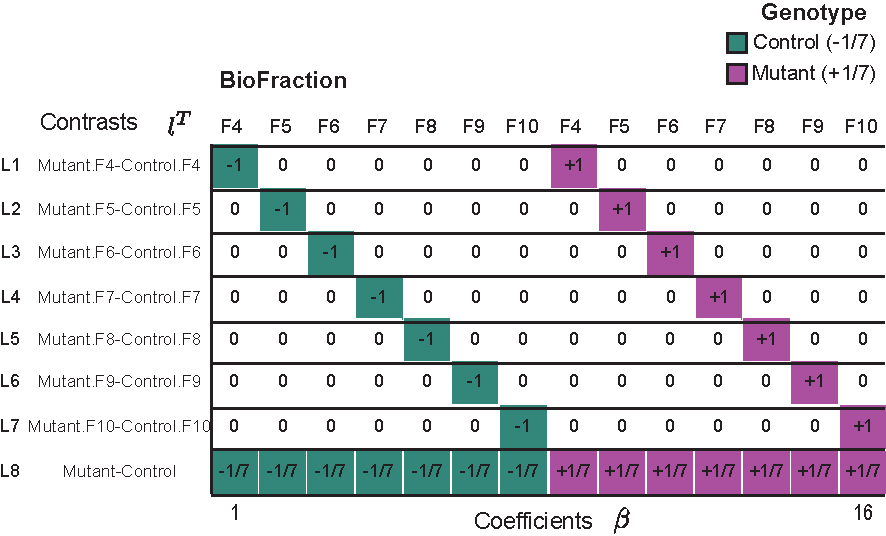
\includegraphics[width=0.9\paperwidth,keepaspectratio]{contrasts}
	  \caption{\textbf{Statistical Comparisons.} We assessed two types of
	  contrasts. Each row of the matrix specifies a contrast between
	  positive and negative coefficients in the mixed-effects model fit to
	  each protein. Contrasts1-7 are intra-BioFraction contrasts that
	  specify the pairwise comparisons of Control and Mutant groups for a
	  single fraction. In Contrast 8 we compare Mutant-Control and assess
	  the overall difference of Control and Mutant conditions.  Each
	  contrast is a vector of sum 1.}
	  \label{fig:contrasts}
  \end{center}
  \end{fullwidth}
\end{figure}

\newpage


\begin{figure}[h] %% figure -- variance
  \begin{fullwidth}
  \begin{center}
	  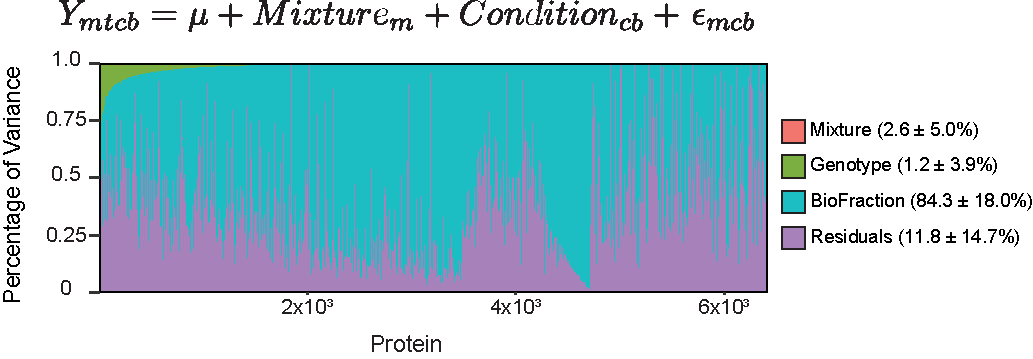
\includegraphics[width=0.9\paperwidth,keepaspectratio]{variance}
	  \caption{\textbf{Analysis of Variance Components.} 
	  The proportion of variance explained by Genotype, BioFraction,
	  Mixture, and remaining residual error (subplot error) for all
	  proteins. Note while the contribution of Mixture seems negligible,
	  its average for all proteins is approximately twice the average
	  percent variance explained by Genotype. BioFraction explains the
	  majority of the variance for all proteins. Analysis done with
	  \texttt{variancePartition::calcVarPart}.}
	  \label{fig:variance}
  \end{center}
  \end{fullwidth}
\end{figure}

\newpage



\end{document}
